%!TEX root = ../main.tex
\section{Conventional argument using the null geodesic}\label{section:conventional}

We are concerned about whether $\Lambda$ contributes to the bending of light around a concentrated mass. Conventional view, first put forth by \citet{Islam1983}, is that it does not, and classical lensing is correct as it is. This view, supported by multiple authors \citep{Lake2002,Finelli2007,Park2008,Simpson2008}, argues that the equations describing the path followed by a photon, the null geodesic equations, takes the same form with or without $\Lambda$ in the Kottler metric. 

The Kottler metric \citep{Kottler1918} represents the Schwarzschild vacuum metric extended to include a cosmological constant. In terms of curvature coordinates ($r$, $\theta$, $\phi$, $t$), the line element in Kottler space is given by

\begin{equation}
  ds^2 = f(r) dt^2 - \frac{dr^2}{f(r)} - r^2 (d \theta^2 + \sin^2 \theta d \phi^2)
  \label{eq:kottler-metric}
\end{equation} 
where 
\begin{equation}
  f(r) = 1 - \frac{2m}{r} - \frac{\Lambda r^2}{3},
  \label{eq:kottler-metric2}
\end{equation}
and $m$ is the mass of the central object and relativistic units ($C = G = 1$) are used. 

There is general agreement \citep{Lake2002,Rindler2007} that when we consider the null geodesic of such a metric, the cosmological constant drops out of the $r$, $\phi$ second-order differential equation in polar coordinates without approximation, and therefore does not contribute to light bending. \citet{Islam1983} found that the differential equation governing light rays moving in a Kottler metric simplifies to

\begin{equation}
  \frac{d^2 u}{d \phi^2} + u = 3mu^2
  \label{eq:null-geodesic-kottler}
\end{equation}
where $u = 1/r$. This formula is independent of $\Lambda$, therefore the resulting solution to this differential equation is the same as in a pure Schwarzschild background. For years this has been the accepted view, supported by the intuition that the cosmological constant is uniform but gravitational lensing occurs as a result of inhomogeneities in the spacetime. 


\section{$\Lambda$ contribution to light bending in Kottler spacetime}\label{section:kottler}

This official opinion was however challenged by \citet{Rindler2007}, who argue that while the $\Lambda$ term drops out of the null geodesic, $\Lambda$ still affects light bending through the metric itself, since the photon is moving in $\Lambda$-dependent geometry. As space is not asymptotically flat, the process of measurement causes the cosmological constant to creep into the light bending angle. 

As noted by \citet{Gibbons2008}, the confusion with the conventional literature lies mainly in the question of what precisely \eqref{eq:null-geodesic-kottler} represents. \eqref{eq:null-geodesic-kottler} merely governs the projection of null rays onto the spatial sections of the metric, but not the more complex geometrical features. Rindler and Ishak's paper attempt to address this. 

They started with the Kottler metric and noted that due to the spherical symmetry of the spatial part of the metric, any orbit must lie entirely in one of the central spatial equatorial coordinate ``plane'' $\theta = \pi / 2$, and in Kottler spacetime this is given by the 2-metric

\begin{equation}
  dl^2 = \left ( 1 - \frac{2m}{r} - \frac{\Lambda r^2}{3}\right )^{-1} dr^2 + r^2 d \phi^2. 
\end{equation}
Without the $\Lambda$ term, this reduces to the Schwarzschild 2-metric. Near the central mass, where the $2m/r$ term dominates over $\Lambda r^2 / 3$, we get the geometry of the upper half of Flamm Paraboloid \citep{Flamm1916}, which has the equation

\begin{equation}
  z^2 = 8m (r - 2m)
\end{equation}
in cylindrical polar coordinates in ordinary 3D Euclidean space. On the other hand, when the $\Lambda r^2 / 3$ term dominates over $2m/r$, we obtain the geometry of a sphere. The Kottler metric is a combination of the two geometries, and the authors are concerned with the region between these two boundaries. 

\begin{figure}
  \centering
  % 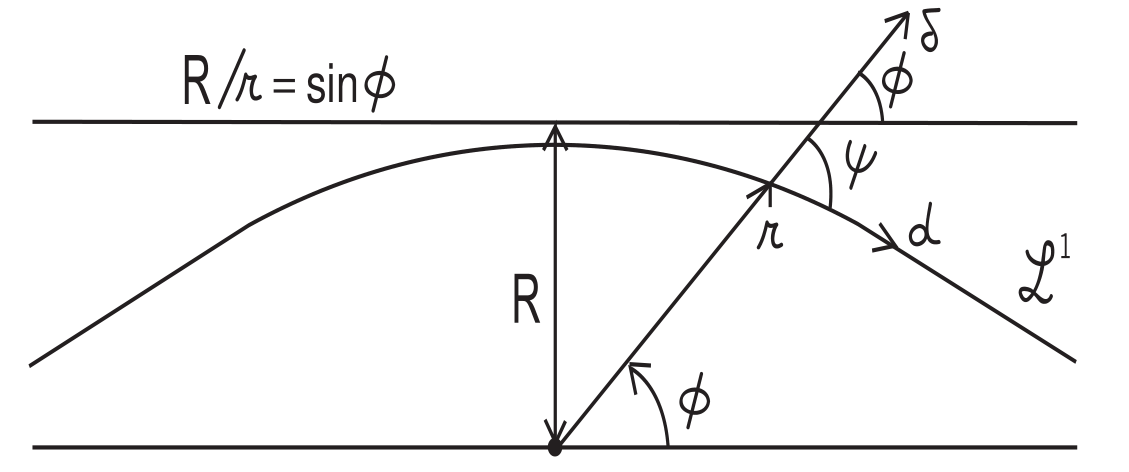
\includegraphics[height=0.5\linewidth]{img/rindler-ishak-2.png}
  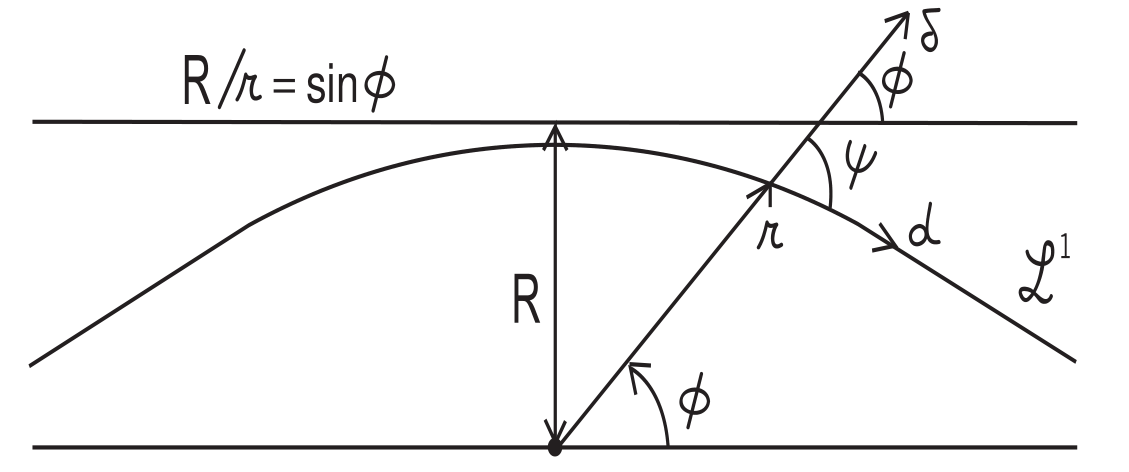
\includegraphics{img/rindler-ishak-2.png}
  \caption{This is the orbital map from \citet{Rindler2007}, describing the plane graph of the orbit equation. The one-sided deflection angle is $\psi - \phi \equiv \epsilon$. }
  \label{fig:rindler-ishak-2}
\end{figure}

Starting with the first approximation of the null geodesic equation \eqref{eq:null-geodesic-kottler}, the authors use the cosine formula for the angle between two coordinate directions

\begin{equation}
  \cos (\psi) = \frac{g_{ij} d^i \delta ^j}{(g_{ij} d^i d^j)^{1/2} (g_{ij} \delta^i \delta^j)^{1/2}}
  \label{eq:cosine-formula}
\end{equation}
to calculate the bending angle $\Psi$ measured by an observer at an arbitrary point $(r, \phi)$ between a ray coming radially from the centre and the ray skirting the lens (see Figure \ref{fig:rindler-ishak-2}). They found that, when the observer and source are equidistant from the lens (i.e. observer is at $\phi = 0$ in Figure \ref{fig:rindler-ishak-2}, arbitrarily chosen), the total light bending angle $\alpha$ to first order in $m / R$ is given by 

\begin{equation}
  \alpha \approx 2 \frac{m}{R} - \frac{\Lambda R^3}{12m}
  \label{eq:rindler-ishak-correction}
\end{equation}
where the first term is simply the classical gravitational lensing bending angle to first order, and the second term is the first order correction to the classical bending angle. 
% As expected from the repulsive nature of $\Lambda$, a positive $\Lambda$ reduces the bending angle. 

The paper by Rindler and Ishak renewed interest in the problem and sparked fresh debate. The authors followed this up with two other papers \citep{Ishak2008b,Ishak2008} that reiterated and elaborated upon their claim. In one of them \citep{Ishak2008b}, they referred to observations of several lensing clusters and showed that the results of these observations do constrain the cosmological constant to within the currently accepted range, and demonstrated potential in their approach to provide another independent constraint on $\Lambda$. 

Their claim was supported by a number of authors \citep{lake2007,Sereno2008,Schucker2008a,Schucker2009}, while questioned by others \citep{Simpson2008,Park2008,Khriplovich2008}. For example, \citet{lake2007} reexamines his previous analysis on the subject \citep{Lake2002} and confirms this dependence. \citet{Schucker2009} finds the same, but notes that further corroboration with observational data is necessary. 

% The dependence was also confirmed by \citet{Sereno2008}, who studied perturbations of the equations of motion in the weak deflection limit using the Kottler metric and provided a general expression from the bending angle. He then derived the lens equation and when evaluated at the same conditions as in the \citet{Rindler2007} paper, he arrived at a cosmological constant term in the deflection, in agreement with \eqref{eq:rindler-ishak-correction}. 

The dependence was also confirmed by \citet{Sereno2008}, who studied perturbations of the equations of motion in the weak deflection limit using the Kottler metric. Using observer coordinates $\{ r_o, \phi_o = 0 \}$ and source coordinates $\{ r_s \phi_s \}$, he wrote down the orbital equation for a light ray from source to observer, and integrated the expression term by term to obtain

% in terms of the first integral of motion $b \equiv \dot{\phi} r^2$ as

% The dependence was also confirmed by \citet{Sereno2008} who later also found a different expression for the dependence on $\Lambda$ \citep{Sereno2008,Sereno2009}. In his paper, Sereno took a slightly different approach and studied perturbations of the equations of motion in the weak deflection limit using the Kottler metric. Using observer coordinates $\{ r_o, \phi_o = 0 \}$ and source coordinates $\{ r_s \phi_s \}$, he wrote down the orbital equation for a light ray from source to observer in terms of the first integral of motion $b \equiv \dot{\phi} r^2$ as

% \begin{equation}
%   \begin{split}
%   \phi_s = \pm \int \frac{dr}{r^2}\left [ \frac{1}{b^2} + \frac{1}{r_{\Lambda}^2} - \frac{1}{r^2} + \frac{2m}{r^3} \right ]^{-1/2}.
%   \end{split}
%   \label{eq:sereno-1}
% \end{equation}

% After some approximations, Sereno integrated \eqref{eq:sereno-1} term by term to obtain

\begin{equation}
  \begin{aligned}
  \phi_s = -\pi  - \frac{4m}{b} + b \left ( \frac{1}{r_s} + \frac{1}{r_o}\right ) - \frac{15 m^2 \pi}{4b^2} - \frac{128m^3}{3b^3} + \frac{b^3}{6} \left ( \frac{1}{r_s^3} + \frac{1}{r_o^3} \right ) - \frac{3465m^4 \pi}{64b^4} \\ - \frac{3584m^5}{5b^5} - \frac{2mb}{r_{\Lambda}^2} - \frac{mb^3}{4} \left ( \frac{1}{r_s^4} + \frac{1}{r_o^4}\right ) + \frac{3b^5}{40} \left ( \frac{1}{r_s^5} + \frac{1}{r_o^5} \right ) - \frac{b^3}{2r^2_{\Lambda}} \left ( \frac{1}{r_s} + \frac{1}{r_o} \right ) + \mathcal{O}(\epsilon^6).
  \end{aligned}
  \label{eq:sereno-2}
\end{equation}
where the cosmological constant appears through terms of order $\mathcal{O}(\epsilon^5)$ and also in $2bm/ r_{\Lambda}^2$. Sereno considered the latter term local since it does not contain positional coordinates of the observer. He then derived the lens equation and when evaluated at the same conditions as in the \citet{Rindler2007} paper, he arrived at a cosmological constant term in the deflection, in agreement with \eqref{eq:rindler-ishak-correction}. 

The limitation of the analysis with Kottler spacetime is that this model assumes a static universe and a point mass as the lens. This is an unrealistic model for practical gravitational lensing since our universe is not static, and neither are gravitational lenses point masses. This may lead to misleading results when drawing conclusions. 
